\documentclass[
  a4paper,
  12pt,
  english,
  brazilian,
]{article}

\usepackage{pdflscape}
\usepackage{pdfpages}
\usepackage[]{fatec-article}
\Author{1}{Name={Davi Mathais\\ Leandro Augusto Muniz\\ Tiago de Lara Rodrigues }}

\Author{2}{Name={\{ davi.almeida3@fatec.sp.gov.br \} \\ \{ leandro.muniz@fatec.sp.gov.br \} \\ \{ tiago.rodrigues39@fatec.sp.gov.br \}}}

\Keyword{1}{Carcinicultura}{Shrimp Farming}
\Keyword{2}{Monitoramento}{Monitoring}
\Keyword{3}{Sustentabilidade}{Sustainability}
\Keyword{4}{Internet das Coisas}{Internet of Things}

\begin{Abstract}[brazilian]
  A carcinicultura é uma atividade de grande relevância econômica e ambiental no Brasil, com destaque para o Nordeste, onde o país se posiciona entre os principais produtores de camarão. Entretanto, a criação enfrenta desafios significativos, como má gestão dos tanques, poluição e maior incidência de doenças, resultando em queda na qualidade do produto. Para mitigar esses problemas e promover práticas sustentáveis, propõe-se um sistema de monitoramento contínuo que integra Arduinos. O sistema acompanha parâmetros essenciais da água, incluindo temperatura, pH e níveis de amônia, e automatiza a alimentação dos camarões de maneira precisa e eficiente. Os dados coletados são armazenados para análises históricas, permitindo melhorias contínuas no manejo dos cativeiros. A plataforma web oferece aos usuários acesso em tempo real aos dados de cada tanque, além de funcionalidades para gerenciamento das informações e controle automatizado da alimentação, garantindo maior comodidade e precisão operacional. Com esses recursos, o sistema busca não apenas aumentar a eficiência produtiva, mas também reduzir impactos ambientais, promovendo uma carcinicultura mais responsável e sustentável.

\end{Abstract}

\begin{Abstract}[english]
  Shrimp farming is an activity of significant economic and environmental relevance in Brazil, with emphasis on the Northeast region, where the country ranks among the leading shrimp producers. However, shrimp farming faces considerable challenges, such as poor pond management, pollution, and higher incidence of diseases, resulting in reduced product quality. To address these issues and promote sustainable practices, a continuous monitoring system integrating Arduinos is proposed. The system monitors essential water parameters, including temperature, pH, and ammonia levels, and automates shrimp feeding in a precise and efficient manner. The collected data are stored for historical analysis, allowing continuous improvements in pond management. The web platform provides users with real-time access to the data from each pond, as well as functionalities for managing information and automated feeding control, ensuring greater convenience and operational accuracy. With these resources, the system aims not only to increase production efficiency but also to reduce environmental impacts, promoting a more responsible and sustainable shrimp farming practice.
\end{Abstract}

\makeindex

\addbibresource{fatec-article.bib}

\begin{document}

\section*{Introdução}%
\label{sect:intro}
\input{Topicos/introducao}

\section*{OBJETIVO}\label{sect:obj}

Este sistema de monitoramento tem como meta desenvolver uma aplicação para auxiliar os produtores criarem camarões de boa qualidade e manter o controle do cativeiro. Dentre os objetivos estão:

\begin{enumerate}

\item Monitorar remotamente os cativeiros, acompanhando pH, temperatura e amônia da água para garantir a qualidade do ambiente e alertar o usuário sobre desvios nos parâmetros.

\end{enumerate}

\section*{Objetivos específicos}

\begin{enumerate}
    \item Registrar e armazenar dados históricos dos cativeiros para possibilitar análises comparativas e avaliação da qualidade ao longo do tempo.

    \item Automatizar o fornecimento de ração, controlando horários e quantidades conforme parâmetros definidos pelo usuário.

    \item Fornecer relatórios e gráficos gerados a partir das informações monitoradas, permitindo uma análise detalhada e fundamentada das condições do cultivo.
    
    \item Cadastrar usuários, cativeiros e pontos de monitoramento, facilitando a gestão e o acesso centralizado às informações.
    
    \item Desenvolver uma aplicação móvel intuitiva e acessível, proporcionando uma experiência prática e eficiente ao carcinicultor.

\end{enumerate}

\section*{ESTADO DA ARTE}\label{sect:estadoarte}

A realização de um sistema de monitoramento para cuidado dos camarões é de grande importância, ajuda tanto o produtor a vender um produto de qualidade, tanto o consumidor que irá consumir algo de qualidade sem prejudicar a sua saúde. Por conta desta importância, é de se imaginar que existam sistemas semelhantes. Dentre os projetos já existentes, há de se destacar determinados artigos.

O trabalho de \cite{dantas2020} propõe um sistema de monitoramento da qualidade da água para a carcinicultura baseado em tecnologias de IoT, utilizando microcontroladores ESP32 integrados a módulos Longo Alcance (do inglês, Long Range, ou LoRa) e sensores de variáveis como pH, oxigênio dissolvido e temperatura. O sistema realiza coleta, processamento e transmissão dos dados via Rede de Longo Alcance e Ampla Cobertura (do inglês, Long Range Wide Area Network, ou LoRaWAN), com integração nos Serviços de Nuvem da Amazon (do inglês, Amazon Web Services, ou AWS) por meio do Protocolo de Telemetria por Enfileiramento de Mensagens (do inglês, Message Queuing Telemetry Transport, ou MQTT). Os resultados mostraram medições precisas de temperatura e pH, com variações mínimas de 0.5°C e comunicação LoRa alcançando cerca de 138 metros, o que se mostrou suficiente para pequenas e médias fazendas. Entre as limitações, destacam-se a necessidade de ampliar o alcance da rede, aprimorar a autonomia energética e incluir novos sensores para um monitoramento mais completo.

O trabalho de \cite{Uddin2020} apresenta um sistema de monitoramento inteligente para fazendas de camarão de água doce baseado em IoT, utilizando sensores conectados a um microcontrolador ESP32 para acompanhar parâmetros como temperatura, pH, salinidade, oxigênio dissolvido e turbidez. Os dados são transmitidos via Wi-Fi para a nuvem e analisados com suporte à decisão baseado na técnica de Processo de Análise Hierárquica (do inglês, Analytic Hierarchy Process, ou AHP) que auxilia na avaliação da qualidade da água e na tomada de decisões pelos produtores. Os testes mostraram alta precisão, sendo eles acima de 93\% e impacto positivo na produtividade, com aumento do tamanho, peso e taxa de sobrevivência dos camarões. Entre as limitações estão a dependência de Wi-Fi, necessidade de calibração periódica e desafios de escalabilidade.

O trabalho de \cite{Zainuddin2019} propõe um sistema de monitoramento da qualidade da água em viveiros de camarão Vannamei utilizando uma rede de sensores sem fio (do inglês, Wireless Sensor Network, ou WSN) integrada à tecnologia IoT. O sistema emprega sensores de temperatura, pH e turbidez conectados a microcontroladores Arduino Atmega 2560 e 328, além de módulos Xbee para comunicação sem fio. Os dados coletados são transmitidos por meio do módulo ESP8266 para uma aplicação web, permitindo o acompanhamento remoto das condições da água. Os testes de calibração demonstraram alta precisão, com índices acima de 97\%, comprovando a eficiência e confiabilidade do sistema. Entretanto, o desempenho depende da estabilidade da conexão de internet e apresenta limitações quanto à expansão para novos sensores e ausência de mecanismos de redundância, o que pode afetar sua escalabilidade e robustez.

Os trabalhos analisados monitoram variáveis como temperatura e pH da água, demonstrando a eficiência da IoT no acompanhamento remoto dos viveiros, mas ainda enfrentam limitações de conectividade, escalabilidade e necessidade de calibração periódica.

Em comparação, o projeto proposto apresenta uma abordagem mais completa, integrando o monitoramento de pH, temperatura e amônia ao controle automatizado da alimentação, com definição de horários e quantidades ideais de ração. Além disso, gera relatórios e gráficos históricos para análise da qualidade da água e desempenho dos cativeiros, e envia alertas preventivos em caso de variações críticas. Assim, diferencia-se por unificar monitoramento ambiental, controle alimentar e apoio à gestão do cultivo em uma única solução.

\section*{METODOLOGIA}\label{sect:metodologia}

O projeto foi desenvolvido com React, para criar interfaces de usuário dinâmicas, e Node.js, que permite executar JavaScript no servidor. Para o back-end, foram utilizadas dependências como Express, para gerenciar rotas e APIs; Cors, para controlar o acesso entre diferentes origens; JWT, para autenticação; e Mongoose, para modelagem e manipulação de dados no MongoDB, um banco de dados NoSQL que permite armazenar informações de forma flexível e escalável. 

O MongoDB foi hospedado no MongoAtlas, plataforma na nuvem que facilita a gestão, segurança e escalabilidade do banco, enquanto o back-end e a API estão no Render, serviço de nuvem para aplicações web, e o front-end no Vercel, plataforma otimizada para deploy rápido e escalável de aplicações web. O sistema foi projetado para uso em dispositivos móveis, oferecendo maior praticidade para o usuário no dia a dia, sendo desenvolvido como Aplicativo Web Progressivo (do inglês, Progressive Web App, ou PWA), que permite que a aplicação funcione como um app nativo, instalação na tela inicial e desempenho otimizado mesmo em navegadores web. 

\section*{Funcionamento do projeto}

No fluxograma apresentado abaixo, é descrito o funcionamento geral do projeto. Na Figura 1, o usuário realiza o cadastro no aplicativo e solicita o cadastramento do cativeiro, necessário para que a equipe responsável realize a instalação dos equipamentos IoT no local.

Na Figura 2, após a autorização do cadastro do cativeiro, o usuário pode acessar todas as informações referentes aos cativeiros, de forma geral ou individual, por meio de um dashboard.

Na Figura 3, todos os dados inseridos na aplicação são enviados para o banco de dados, que armazena as informações e as disponibiliza para visualização pelo usuário. Além disso, o banco de dados envia os dados coletados para o equipamento IoT, conforme mostrado na Figura 4.

Na Figura 4, o equipamento IoT, representado pelo ESP32, utiliza seus sensores de temperatura, pH e amônia para captar os dados do cativeiro e enviá-los ao banco de dados, garantindo que o usuário tenha acesso às informações coletadas em tempo real.

Na Figura 5, os dados enviados do banco de dados também são encaminhados para o dispensador de ração, contendo informações sobre o horário e a quantidade de alimento. O dispenser armazena essas instruções e realiza a alimentação no momento programado pelo usuário. Após a alimentação, um alerta é enviado ao aplicativo, informando que o procedimento foi realizado com sucesso.

\begin{figure}[!htb]
\SetCaptionWidth{\ifbool{@LayoutA}{0.7}{0.72}\linewidth}
\caption{Fluxograma sobre funcionamento do sistema}%
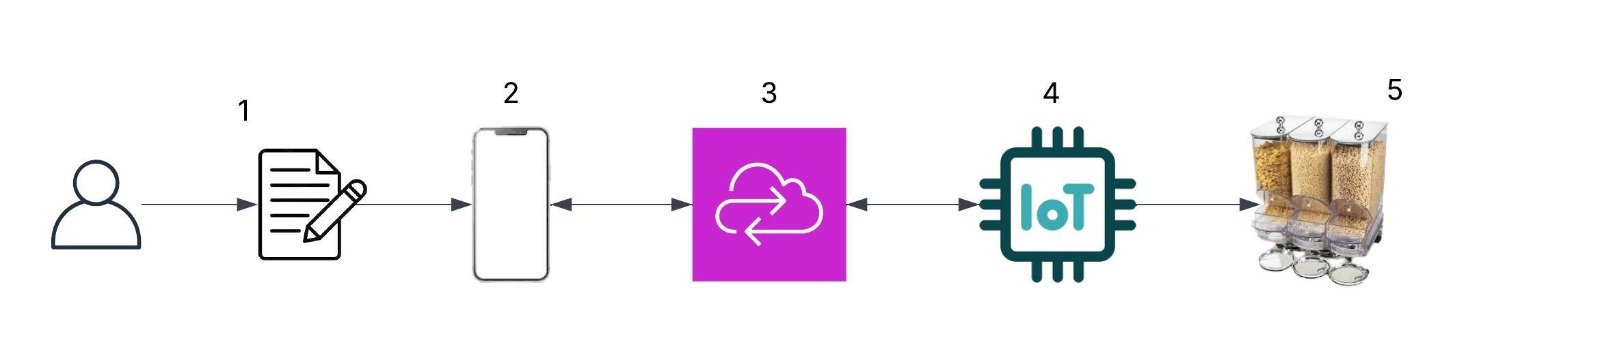
\includegraphics[width = 1.55\CaptionWidth]{Imagem/Fluxograma.jpeg}
\SourceOrNote{Autoria Própria}
\end{figure}

\section*{RESULTADOS PRELIMINARES}\label{sect:resultados}

Esta seção será dedicada à apresentação e análise dos resultados obtidos a partir da aplicação da metodologia escolhida. No momento, encontra-se em fase de construção. 
A versão final incluirá dados organizados em tabelas, gráficos ou outras formas de representação, acompanhados de interpretações fundamentadas. O conteúdo será desenvolvido assim que forem concluídas as etapas práticas do projeto, permitindo a coleta e sistematização das informações relevantes.

\section*{CONCLUSÃO}\label{sect:conclusao}

A Conclusão será elaborada após a finalização das etapas de desenvolvimento e análise dos resultados. Este espaço será utilizado para apresentar as principais reflexões e aprendizados do grupo, destacando a relevância do trabalho, suas contribuições e possíveis desdobramentos. Como o projeto ainda está em andamento, esta seção permanece em aberto e será preenchida com base nas evidências e interpretações construídas ao longo do processo investigativo.

\newpage

\printbibliography

\end{document}